\subsection{Profile Likelihood Ratio}

The procedure for setting exclusion limits using the likelihood function 
(Eq.\ref{eq:stat.like.Pr})
relies on a profile-likelihood-ratio test~\cite{Cowan:2010js}.
The null hypothesis considered is that of background only with $\mu=0$ and the alternate hypothesis 
is the presence of a signal with strength $\mu>0$.
According to the Neyman-Pearson Lemma \cite{Neyman289}, 
the most powerful test when performing a hypothesis test between two simple hypotheses, $\mu=0$ and $\mu>0$,
is the profile-likelihood-ratio test, which rejects $\mu=0$ in favor of $\mu>0$.
%Important advantage of profile LR is that its distribution becomes independent of nuisance parameters in large sample limit.
The profile-likelihood-ratio test $q_{\mu}$ is defined to be
\begin{equation}
q_{\mu}  \left( \vect{X} \right)= 
\begin{cases}
  -2\ln\left(
  \frac
      {\mathcal{L} \left( \mu, \hat{\hat{\vect{\theta}}}\left(\mu\right) \rvert \vect{X} \right)}
      {\mathcal{L} \left( \hat{\mu}, \hat{\vect{\theta}} \rvert \vect{X} \right)}
 \right), & \text{if}\ \mu > \hat{\mu} \\
      0, & \text{otherwise}
    \end{cases}
\label{eq:stat.limit.qmu}
\end{equation}
For a given observation $\vect{X}$, the parameters $\hat{\mu}$ and $\vect{\theta}$ are obtained from maximizing the likelihood. 
If the value of $\mu$ is also fixed, the set of values $\hat{\hat{\vect{\theta}}}$ corresponds to the set of values that 
maximize the likelihood for that particular value of $\mu$. The variable $q_{\mu}$ is always positive ($q_{\mu}\geq0$).
Qualitatively, small values of $q_{\mu}$ correspond to a better compatibility between the observed data and the 
tested hypothesis with a signal strength $\mu$, while large values indicate a very improbable signal hypothesis.
The condition on the sign of $ \mu - \hat{\mu}$ is necessary in order not to interpret an upward fluctuation of data 
($X > \mu s + b$) as incompatible with the tested hypothesis. 
The form of $q_{\mu}$ is motivated by Wald and Wilk's \cite{Wilks:1938dza,Wald:ams1943} approximation formulas in the large sample limit
where the distributions of $q_{\mu}$ also become independent of nuisance parameters as it will be discussed next.
The test statistic for discovery will try to reject the background only hypothesis ($\mu=0$). Thus Eq.\ref{eq:stat.limit.qmu} becomes
\begin{equation}
q_{0}  \left( \vect{X} \right)= 
\begin{cases}
  -2\ln\left(
  \frac
      {\mathcal{L} \left( 0, \hat{\hat{\vect{\theta}}}\left(0\right) \rvert \vect{X} \right)}
      {\mathcal{L} \left( \hat{\mu}, \hat{\vect{\theta}} \rvert \vect{X} \right)}
 \right), & \text{if}\ \hat{\mu} < 0 \\
      0, & \text{otherwise}
    \end{cases}
\end{equation}

\subsection{The $p$-value}

At this stage, a test statistic $q_{\mu}$ has been constructed to distinguish between the hypothesis 
that the data contains signal and background $\mu>0$ and that of background only $\mu=0$.
To illustrate the limit setting procedure, we consider distributions of the test statistic under each 
hypothesis: $f\left(q_{\mu} \rvert \mu\right)$ for $\mu>0$ and $f\left(q_{0} \rvert 0\right)$ for $\mu=0$.
These distributions are shown in Figure~\ref{fig:stat.limit.qmunormal} and details on how to obtain their functional forms
 will be discussed later. 

\begin{figure}[t]
\centering
\begin{subfigure}[t]{0.45\textwidth}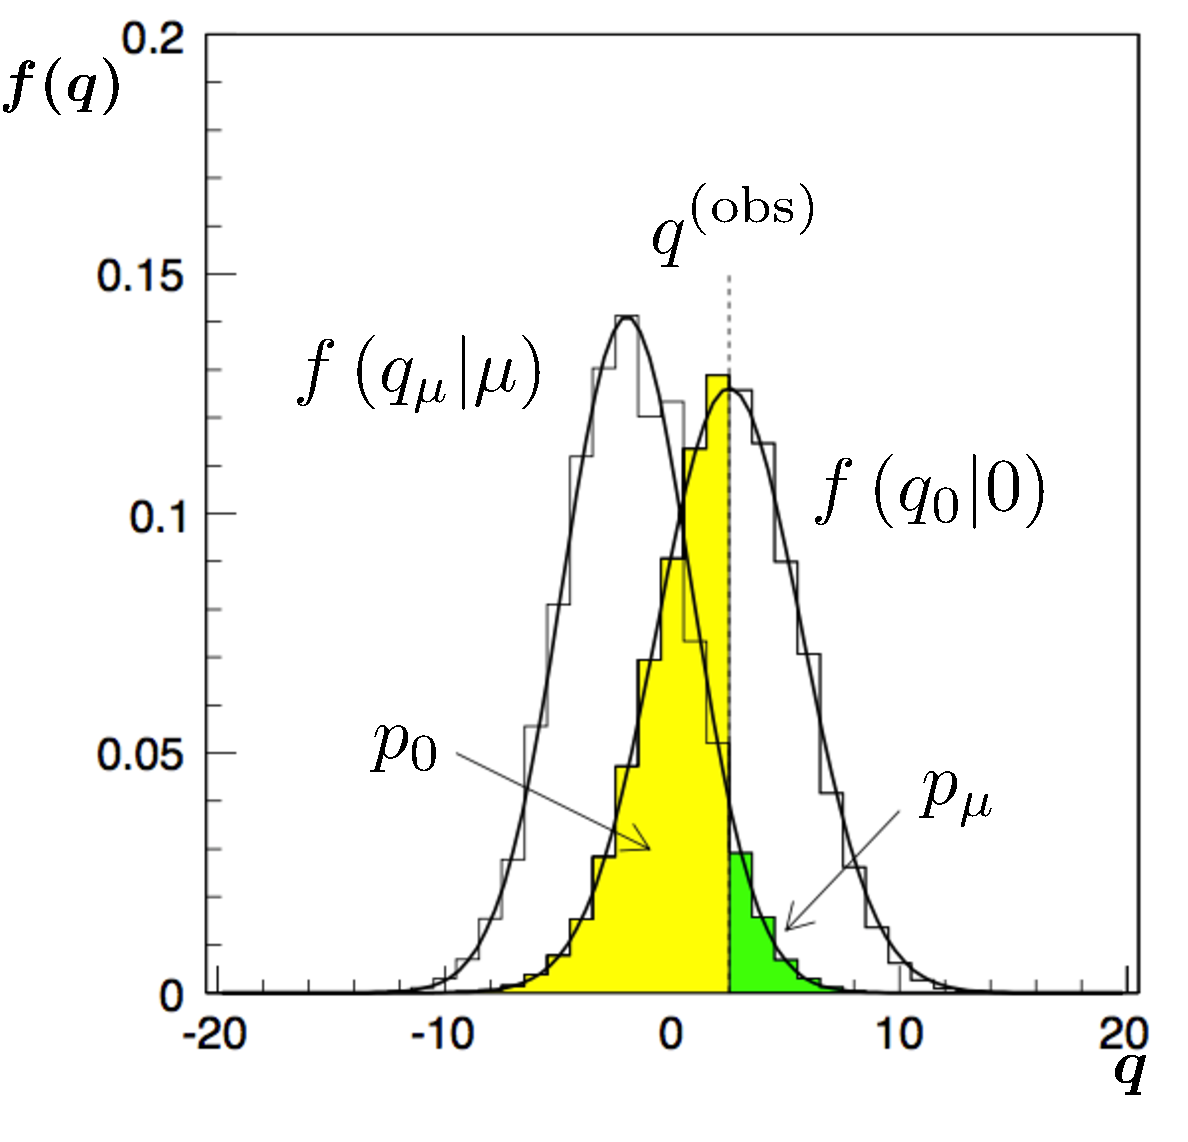
\includegraphics[width=\textwidth]{qmunormal}\caption{}\label{fig:stat.limit.qmunormal}\end{subfigure}
\begin{subfigure}[t]{0.467\textwidth}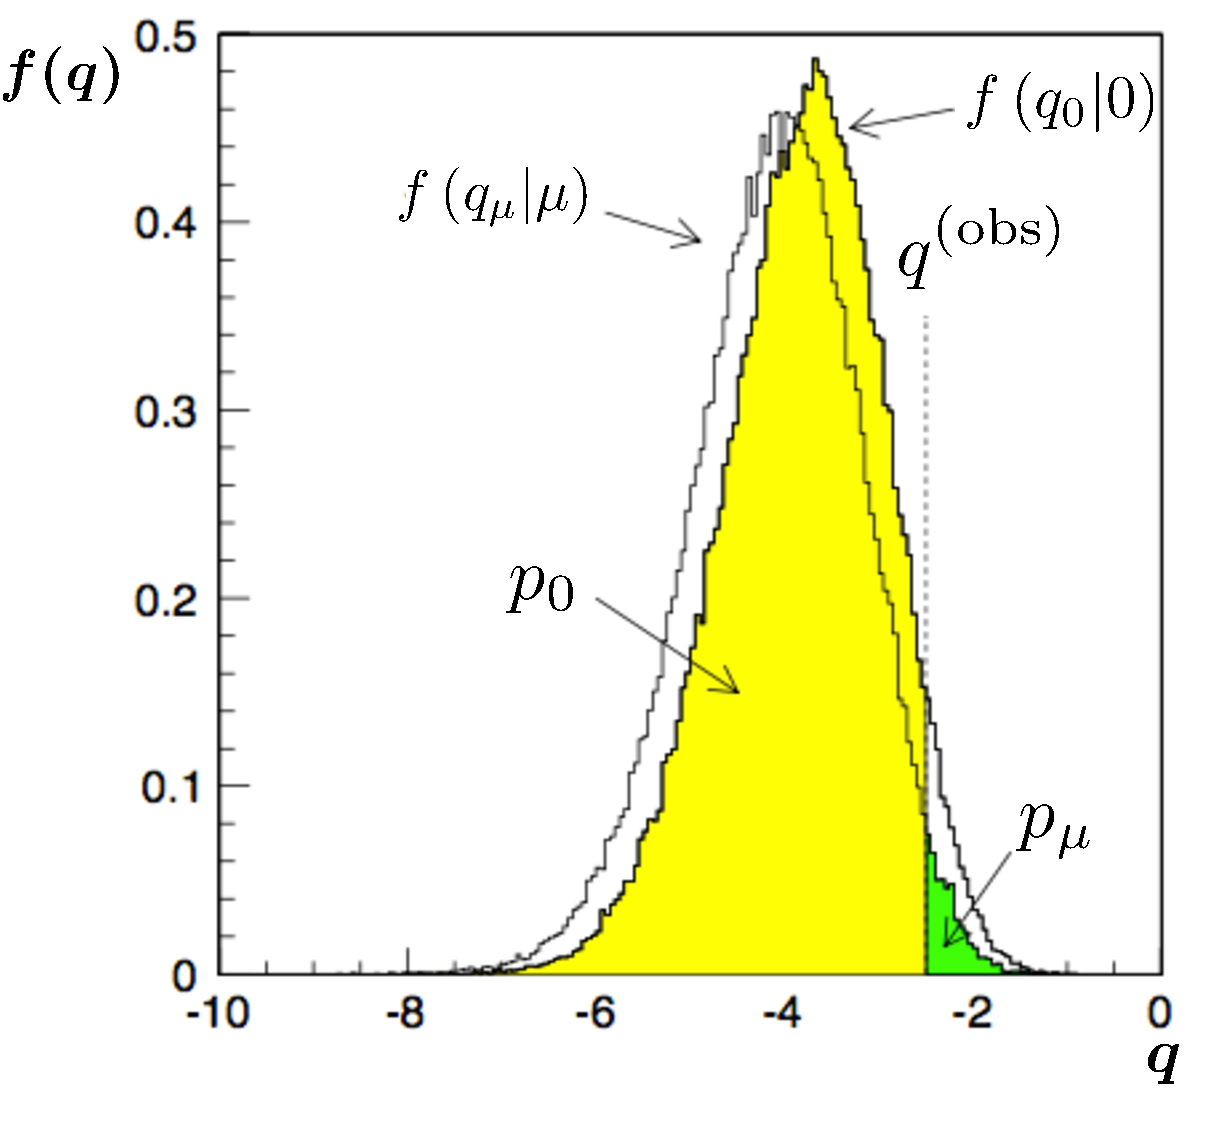
\includegraphics[width=\textwidth]{qmunosens}\caption{}\label{fig:stat.limit.qmunosens}\end{subfigure}
\caption{Distributions of the test variable $q_{\mu}$ under the $\mu>0$ and $\mu=0$ hypotheses: (a) typical case, 
  (b) case where there is very little sensitivity to the signal model}
\label{fig:stat.limit.qmu}
\end{figure}

Given that the actual observed data leads to a test variable $q_{\mu}^{\left(\text{obs}\right)}$, it is possible to 
quantify the level of discrepancy between the observed data and the tested hypothesis ($\mu>0$ or $\mu=0$) using 
a $p$-value. 
The $p$-value of the signal hypothesis ($\mu>0$) is then defined as the probability, under assumption of the signal hypothesis, 
to find a value of $q_{\mu}$ with equal or lesser compatibility with the signal model considered relative to what is 
found with $q_{\mu}^{\left(\text{obs}\right)}$. In other words,  higher values of $q_{\mu}$ indicate an increasing disagreement
between data and the signal model. The mathematical expression of the $p$-value with $\mu>0$ is taken as the probability 
to find $q_{\mu}$ greater than or equal $q_{\mu}^{\left(\text{obs}\right)}$, under the signal hypothesis\footnote{Note that 
 the background-only distribution $f\left(q_{0} \rvert 0\right)$ in the example given in 
Figure~\ref{fig:stat.limit.qmunormal} is shifted to the right.} is given by
\begin{equation}
p_{\mu} = \Pr\left(q_{\mu} \geq q_{\mu}^{\left(\text{obs}\right)} \rvert \mu \right) = \int_{q_{\mu}^{\left(\text{obs}\right)}}^{\infty} f\left(q_{\mu} \rvert \mu\right) \diff q_{\mu}
\end{equation}
where $q_{\mu}^{\left(\text{obs}\right)}$ is the value of the statistic test observed in data and the function $f$
denotes the probability distribution function of $q_{\mu}$ under the signal hypothesis. 
Similarly, the $p$-value of the background-only hypothesis with $\mu=0$ takes the form of 
\begin{equation}
p_{0} = \Pr\left(q_{0} \geq q_{0}^{\left(\text{obs}\right)} \rvert 0 \right) = \int^{q_{0}^{\left(\text{obs}\right)}}_{-\infty} f\left(q_{0} \rvert 0\right) \diff q_{0}
\end{equation}
and can be interpreted as the probability of the observation to be consistent with the background only hypothesis:
the smaller the $p_{0}$ value is, the less compatible data is with the background only hypothesis. 
In order to claim a discovery in particle physics, 
the background-only hypothesis must be rejected using the $p_0$-value. 
However, there is an ambiguity related to how small the $p_0$-value needs to 
be, before declaring a discovery. 
The problem can also be formulated in terms of significance.
Assuming a Gaussian distributed variable, how many $Z$ standard deviations 
$\sigma$ above the mean are required to cover an upper-tail probability equal 
to $p$ expressed as 
\begin{equation}
Z = \Phi^{-1}\left(1-p\right)
\end{equation}
 where $\Phi$ is the Gaussian cumulative distribution.
The particle physics community considers a discovery if $Z=5$, commonly 
used ``five sigma excess'' statement, which corresponds to 
$p_0 = 2.87\times 10^{-7}$ or one in 3.5 million probability for the background
 to be as extreme as the observation. In order to announce evidence for a 
new particle, a significance of $Z=3$ or $p_0 = 1.35\times 10^{-3}$ is required.


\subsection{The $CL_\mathrm{s}$ Prescription}
The next step is to define a confidence interval ($CI$) that includes the parameter $\mu$ at a specified confidence level ($CL$). 
In other words, instead of estimating the parameter $\mu$ by a single value, an interval $CI$ likely to include the parameter is given.
The $CL$ provides a quantitative statement on how likely the interval $CI$ is to contain the parameter $\mu$. 
If given the measurement of a parameter $\mu_{meas}$, we deduce that there is a 95\% $CI$ $[\mu_1,\mu_2]$ means 
that in an ensemble of experiments 95\% of the obtained $CI$s will contain the true value of $\mu$.
The upper limit is simply the case where the 95\% $CI$ is $[0,\mu_{up}]$:
In an ensemble of experiments 95\% of the obtained $CI$s will contain the true value of $\mu$, including $\mu=0$. 
The conclusion is that $\mu < \mu_{up}$ at the 95\% $CL$ or that $ \mu_{up}$ is an upper limit. 

Applying this concept to the problem at hand where we want to place an upper limit on the expected number of 
signal events $S$ ($S=\mu s$, $s$ being the expected number of signal events for $\mu=1$) in one or more signal regions.
The $CL$ is obtained from a standard statistical test of the signal model ($\mu>0$) which can establish the exclusion of the signal 
model at confidence level $1-\alpha = 95 \%$ if 
\begin{equation}
  CL_\mathrm{s+b}  = p_{\mu} < \alpha
\end{equation}
where $\alpha=0.05$. 
Since the result section will present $CL$ values in terms of the expected number of signal events from beyond the standard model 
processes, we continue this discussion of estimating an upper limit on $S$ rather than $\mu$.
Thus, a $CI$ at confidence level $CL=1-\alpha$ for the expected number of signal events $S$ can be constructed from those values of
$S$ (or $\mu$) that are not excluded, and the upper limit $S_{up}^{1-\alpha}$ is the largest value of $S$ not excluded.
By construction, the interval $[0,S_{up}^{95}]$ will cover the expected number of signal events $S$ with a probability of at least 
95\%, regardless of the value of $S$.

An anomaly arises with the $CL_\mathrm{s+b}$ prescription when the number of expected signal events is much less than that of 
the background and the data observation had a downward fluctuation below the expected background.
The procedure will lead to excluding, with probability close to $\alpha$, hypotheses to which the experiment has no sensitivity.
For $\alpha=5\%$, it means that one out of twenty tests for different signal models where one has no sensitivity will result in exclusion.
In fact, the desired behavior of the exclusion probability in this case is to approach zero rather than $\alpha$.
This scenario is illustrated in Figure~\ref{fig:stat.limit.qmunosens} where the distribution of $q_{\mu}$
under both the signal and background-only hypotheses are almost similar. 
To remedy this problem, a different procedure is used where a model is regarded as excluded if 
\begin{equation}
  CL_\mathrm{s}  = \frac
{p_{\mu}}
{1-p_{0}}
%  {\Pr\left( q_{\mu} \geq q_{\mu}^{\left(\text{obs}\right)}\rvert \mu \right)}
%  {\Pr\left( q_{\mu} \geq q_{\mu}^{\left(\text{obs}\right)}\rvert \mu = 0 \right)}
< \alpha.
\end{equation}
In this form, the $p$-value is penalized by dividing by $1-p_{0}$. 
If the distribution of $q_{\mu}$ under signal or background-only hypotheses are widely separated, then 
the quantity $1-p_{0}$ is close to unity which recovers the $CL_\mathrm{s+b}$ value. However, if
the distributions of both hypotheses are similar, due to the lack of sensitivity, $1-p_{0}$ becomes smaller
and the $CL_\mathrm{s+b}$ value is increased more leading to a weaker upper limit. 
Similar to the case of $CL_\mathrm{s+b}$, the upper limit on $S_{up}^{95}$ is taken as the largest value of the parameter
$S$ not excluded.

\subsection{Approximate Sampling Distributions}

The remaining task is to determine the sampling distributions
$f\left(q_{0} \rvert 0\right)$ and $f\left(q_{\mu} \rvert \mu\right)$
needed to compute the $p$-values
used in the case of discovery and setting upper limits, respectively.
These distributions do not have an analytic form but can be obtained from 
pseudo-experiments or asymptotic approximations.
The pseudo-experiments are more accurate than the asymptotic 
approximations since a large number of 
datasets are generated which are drawn from a distribution that is consistent 
with those observed.
However, for a complex likelihood function where the procedure of generating 
pseudo-datasets needs to be repeated many times for each parameter point
of each model being considered, the pseudo-data set method is computing 
intensive and not practical. For this reason, the current analysis 
uses asymptotic formulae to approximate $q_{\mu}$ and shown to be valid in the 
large sample size limit \cite{Cowan:2010js}. The approximation is based on an important result 
by Wilks \cite{Wilks:1938dza} and Wald \cite{Wald:ams1943} who showed that for a single parameter of interest,
\begin{equation}
  q_{\mu} =
  \begin{cases}
    \frac{\left(\mu - \hat{\mu}\right)^2}{\sigma^2} + \mathcal{O}\left(\frac{1}{\sqrt{N}}\right)
    , & \text{if}\ \mu > \hat{\mu} \\
    0, & \text{otherwise}.
  \end{cases}
\label{eq:stat.model.asymp}
\end{equation}
where $\mu$ is a Gaussian distribution with a mean $\bar{\mu}$ and 
standard deviation $\sigma$, and a sample size $N$. In the case where 
$\mu = \hat{\mu}$, the test statistic $q_{\mu}$ follows a $\chi^2$ distribution
with one degree of freedom. 
The variance $\sigma^2$ is obtained from an artificial data set called the 
``Asimov data set''
\footnote{Inspired from the short story \textit{Franchise}\cite{asimov} by Isaac Asimov that entails replacing a single voter that represents the entire electorate 
population in an election. Similarly, an ensemble of pseudo-experiments 
can be replaced by a single representative data set.}
 that verifies $X_A = \bar{\mu} s + b$. 
From Eq.\ref{eq:stat.model.asymp}, the variance is then 
$\sigma^2 = \left( \mu - \bar{\mu} \right)^2/q_{\mu,A}$, where $q_{\mu,A}$ 
is evaluated from the exact expression of $q_{\mu}$ using the Asimov data set.

The results obtained from the asymptotic approximations have been compared to 
exclusion limits obtained with a limited number of pseudo-experiments.
A reasonable agreement has been observed which validated the use of 
the asymptotic formalism to obtain the exclusion limits on the different models.
